\documentclass[12pt,letterpaper]{article}
\usepackage[utf8]{inputenc}
\usepackage[spanish]{babel}
\usepackage{amsmath}
\usepackage{amsfonts}
\usepackage{amssymb}
\usepackage{graphicx}
\usepackage{lmodern}
\usepackage{kpfonts}
\usepackage{fourier}
\usepackage{color}
\usepackage{listings}
\usepackage{hyperref}
\usepackage{multicol}
\usepackage{multirow, array}
\usepackage{enumerate}
\usepackage[left=2.5cm,right=2cm,top=2cm,bottom=2cm]{geometry}
\usepackage{float}
\usepackage{fancyhdr}
\usepackage{quotchap}
\usepackage{tikz}
\usepackage[hidelinks]{hyperref}
\usepackage{chemfig}
\usepackage{pgfplots}
%\usepackage{color}      % Definición de colores
%    \hypersetup{colorlinks=true, linkcolor=[rgb]{0,0,1}, citecolor=[rgb]{0,0,1}}
\usepackage{xcolor}		% Permite definir un color para utilizarlo dentro del documento.
%    \definecolor{gris}{RGB}{70,70,70}	    % Definiendo el color gris
%    \definecolor{negro}{RGB}{40,40,40}		% Definiendo el color negro

%%%%%%%% Modificación de los espacios de los títulos de secciones %%%%%%%%%%
\usepackage{titlesec}		% Permite reconfigurar  los títulos de las secciones y subsecciones
%% =============================================================================
%%  OTRA COSA QUE NO SEAN PAKETES
%% =============================================================================
\pagestyle{fancy}
\setcounter{secnumdepth}{3}
\setcounter{tocdepth}{4}
\fancyhf{}
\rhead{I5839 D-03}
\lhead{Laboratorio de reactores(2020B)}
\rfoot{\thepage}
%\renewcommand\thesection{\Roman{section}}	% Numeración romana en las secciones
%\renewcommand\thesubsection{\Roman{subsection}}		% Numeración romana en las subsecciones
\titlespacing*{\section}{0pt}{2.5mm}{0mm}	% Espaciado del título {espacio izquierdo}{arriba del título}{abajo del título}
\titleformat{\section}[block]{\large\scshape\centering}{\thesection.}{1em}{}
\titleformat{\subsection}[block]{\large}{\thesubsection.}{1em}{}
%\newcommand{\colorhrule}[3]{\begingroup\color{#1}\rule{#2}{#3}\endgroup}

\setlength{\intextsep}{1mm} % Distancia superior e inferior en objetos flotantes
\setlength{\columnsep}{5mm} % Separación entre columnas del documento
\spanishdecimal{.}
%% =============================================================================
%%    INICIO DEL DOCUMENTO
%% =============================================================================
\begin{document}
\renewcommand{\tablename}{Tabla}
\thispagestyle{empty}
%======================
%       PORTADA
%======================
\sloppy     % Evita que las palabras se corten al saltar de línea.
\begin{center}
  \begin{tabular}{cc}

\multirow{2}{3.5cm}{
\includegraphics[width=3cm]{Figuras/udg.pdf}}	& \huge{\textsc{\textbf{Universidad de Guadalajara}}}\\
 & \scriptsize{\textsc{CENTRO UNIVERSITARIO DE CIENCIAS EXACTAS E INGENIERÍAS}}\\[5mm]
 & \Large{\textsf{\textbf{Práctica 4. Distribución de tiempos de residencia
}}}\\
 & \\ \vspace{5mm}
 & \small{\textsf{Alejandro Leviatán Gallifrey  [213521903]}}\\
 & \small{\textsc{Ingeniería Química $|$  - Laboratorio de reactores Químicos}}\\
 & \today\\
 & \small{\textit{Profersor:}}  \textbf{\small{Alejandro Nava Tellez }}\\
  \end{tabular}
\end{center}

%\begin{center}
 % \colorhrule{negro}{16.5cm}{1.2pt}
%\end{center}

\rule{\linewidth}{0.75mm}

\tableofcontents
A partir de observaciones experimentales, Arrhenius estableció la dependencia que la
constante de velocidad específica de una reacción tiene con la temperatura:
\[k=A exp \left( \frac{-E_{a}}{RT}\right ) \]
Donde $k$ es la constante de velocidad, $A$ el denominado factor de frecuencia, $E_a$ la
energía de activación, $R$ la constante de los gases y $T$ la temperatura expresada en
Kelvin. Si se realizan experimentos a diferentes temperaturas, se pueden determinar
los parámetros $A$ y $E_a$ a partir de la representación lineal de la ecuación de Arrhenius
en su forma logarítmica:
$$ ln k =ln A - \dfrac{E_a}{R} \dfrac{1}{T} $$
%
%
%
\section{Objetivos}
  \justify
Analizar el efecto de la temperatura y determinar los parámetros de la ecuación de
Arrhenius: energía de activación y factor de frecuencia.
%
%
%
\section{Prerreporte}
    \begin{enumerate}
        \item ¿Cuáles son las características de una reacción exotérmica y de una endotérmica?
        \begin{itemize}
            \item Exotérmica:
        \end{itemize}
        Durante una reacción exotérmica el calor \textit{sale} o fluye \textit{hacia afuera} del sistema, es decir, hacia el entorno.

        $$\Delta H<0$$
        \begin{itemize}
            \item Endotérmica:
            \end{itemize}
            Durante una reacción endotérmica, el calor fluye \textit{hacia dentro} del sistema desde su entorno.

            $$\Delta H>0$$
        \item Que representan el factor de frecuencia y la enería de activación.
        \begin{itemize}
            \item Factor de frecuencia:
        \end{itemize}
        El factor de frecuencia "\textit{A}" es una relación empírica entre la temperatura y el coeficiente de velocidad.

        \begin{itemize}
            \item Energía de activación:
        \end{itemize}
         Es la energía mínima que necesita un sistema antes de poder iniciar la reacción.

        \item  ¿Cuál es el efecto de la temperatura en una reacción química?

        La temperatura influye directamente en la velocidad de reacción. Mientras mayor sea la temperatura mayor es el número de choques entre las moléculas y mayor la velocidad de la reacción.
    \end{enumerate}

    \subsection{Materiales y reactivos}
    \justify
    Para el desarrollo de esta práctica se requiere un reactor esférico con 3 bocas esmeri-
ladas de 250 mL, un soporte universal, una pinza de 3 dedos, dos tapones de hule, un condensador, manguera, un cronómetro y dos probetas de 100 mL, 2 vasos de precipitados de 100 mL, una propipeta, un conductímetro, una pizeta, dos matraces aforados de 100 mL, una espátula, un termómetro, un agitador magnético y una barra de agitación magnética. Además se requieren 100 mL de una solución de 0.2 M de NaOH y 100 mL de una solución 0.2 M de acetato de etilo. Y también se necesita
%
%
%
    \subsection{Procedimiento}
      \justify
    Preparar las soluciones de NaOH y de acetato de etilo. En el reactor perfectamente
limpio y seco, colocar 100 mL de solución de NaOH 0.2 M. Fijar el reactor al soporte
universal e introducir en el baño térmico ajustando la temperatura de reacción. Medir
con la probeta 100 mL de acetato de etilo y vaciarlos a un vaso de precipitados. Colocar
el termómetro y el conductimetro en el reactor. Vaciar la solución medida de acetato
de etilo al reactor, agitar vigorosamente durante unos segundos con ayuda del agitador
magnético y poner en marcha el cronómetro. Hacer medidas de conductividad para la
reacción a los siguientes tiempos: 0.5, 1, 1.5, 2, 3, 5, 7, 10, 13 y 18. Una vez realizadas
las mediciones anteriores, vaciar la muestra en un frasco de vidrio, cierre y deje enfriar
a temperatura ambiente. Este procedimiento se deberá realizar para las siguientes
temperaturas: 35, 50, 65 y 80 $^{\circ}$C. Deberán obtenerse las curvas de calibración a cada
temperatura.
    \subsection{Diagrama}
        \begin{figure}[H]
            \centering
            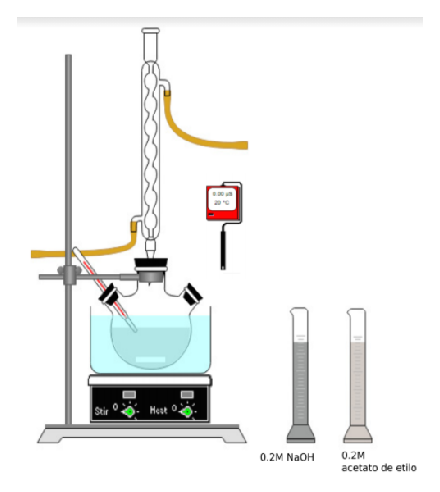
\includegraphics[scale=0.7]{Figuras/Diagrama.eps}
            \caption{Diagrama de la pr\'{a}ctica}
        \end{figure}
%
%
%
\section{Cálculos}


\begin{enumerate}
        \item Expresar la ley de velocidad para la reacción.
         Para este caso $ A$ es acetato de etilo y $B$ es el Hidróxido de sodio.

                $$ -r_{a}= k[A][B] $$
        \item Elaborar una gráfica de conductividad en función del tiempo y extrapolar a t = 0.
\end{enumerate}




     \begin{figure}[H]
         \centering
         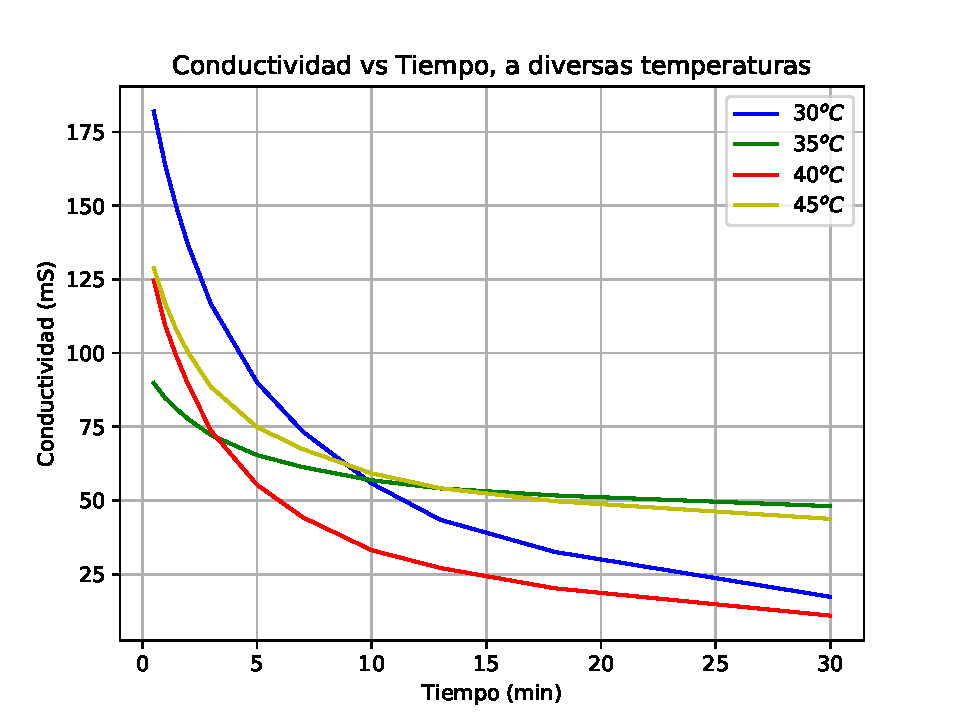
\includegraphics[scale=1]{Figuras/Conductividad_vs_Tiempo.pdf}
         \caption{Diagrama de la pr\'{a}ctica}
      \end{figure}
%

%\begin{commet}
\begin{figure}[H]
    \centering
    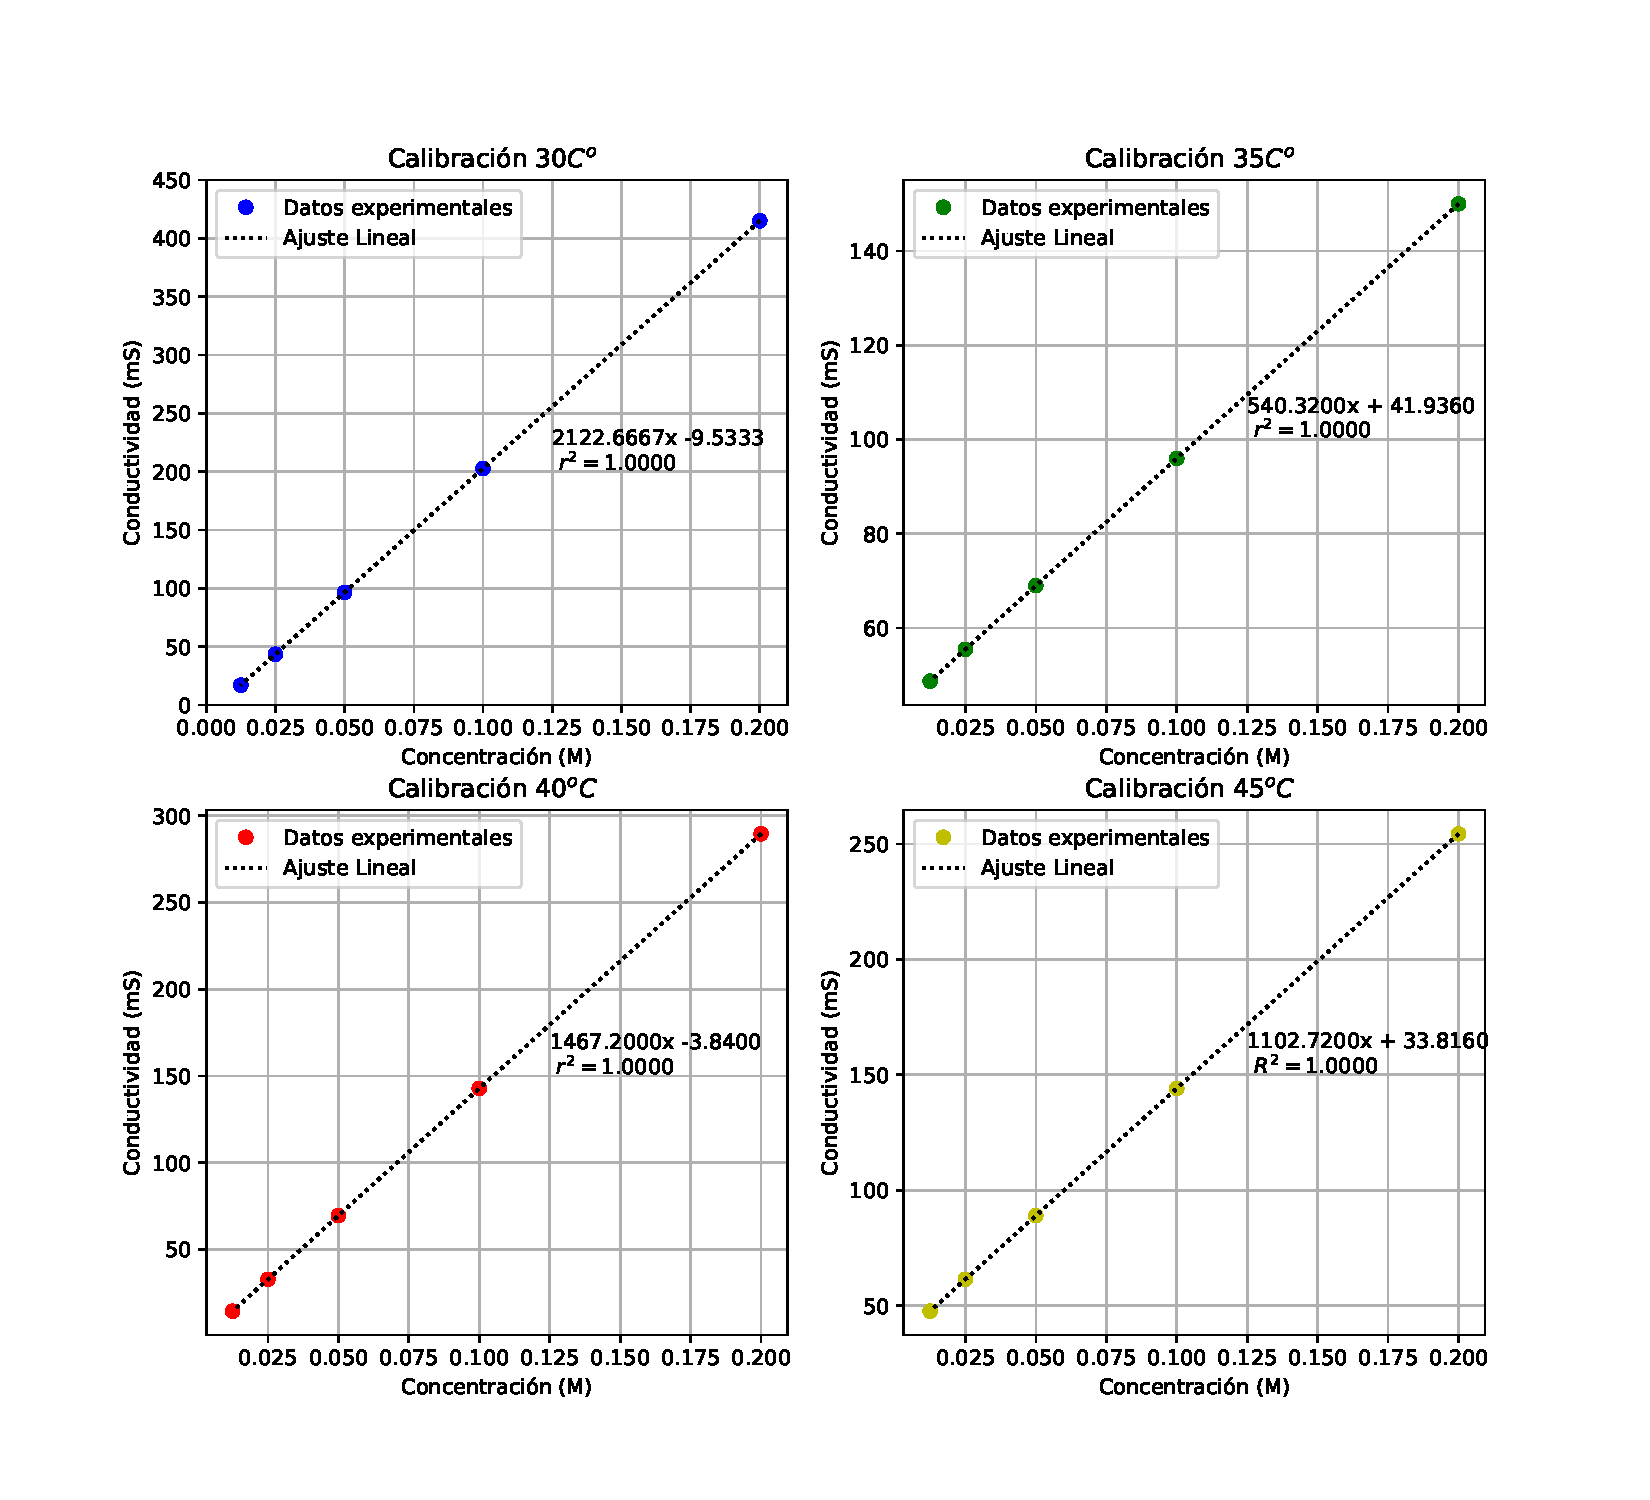
\includegraphics[scale=0.65]{Figuras/FiguraTodos.pdf}
    \caption{Diagrama de la pr\'{a}ctica}
\end{figure}

\begin{figure}[H]
    \centering
    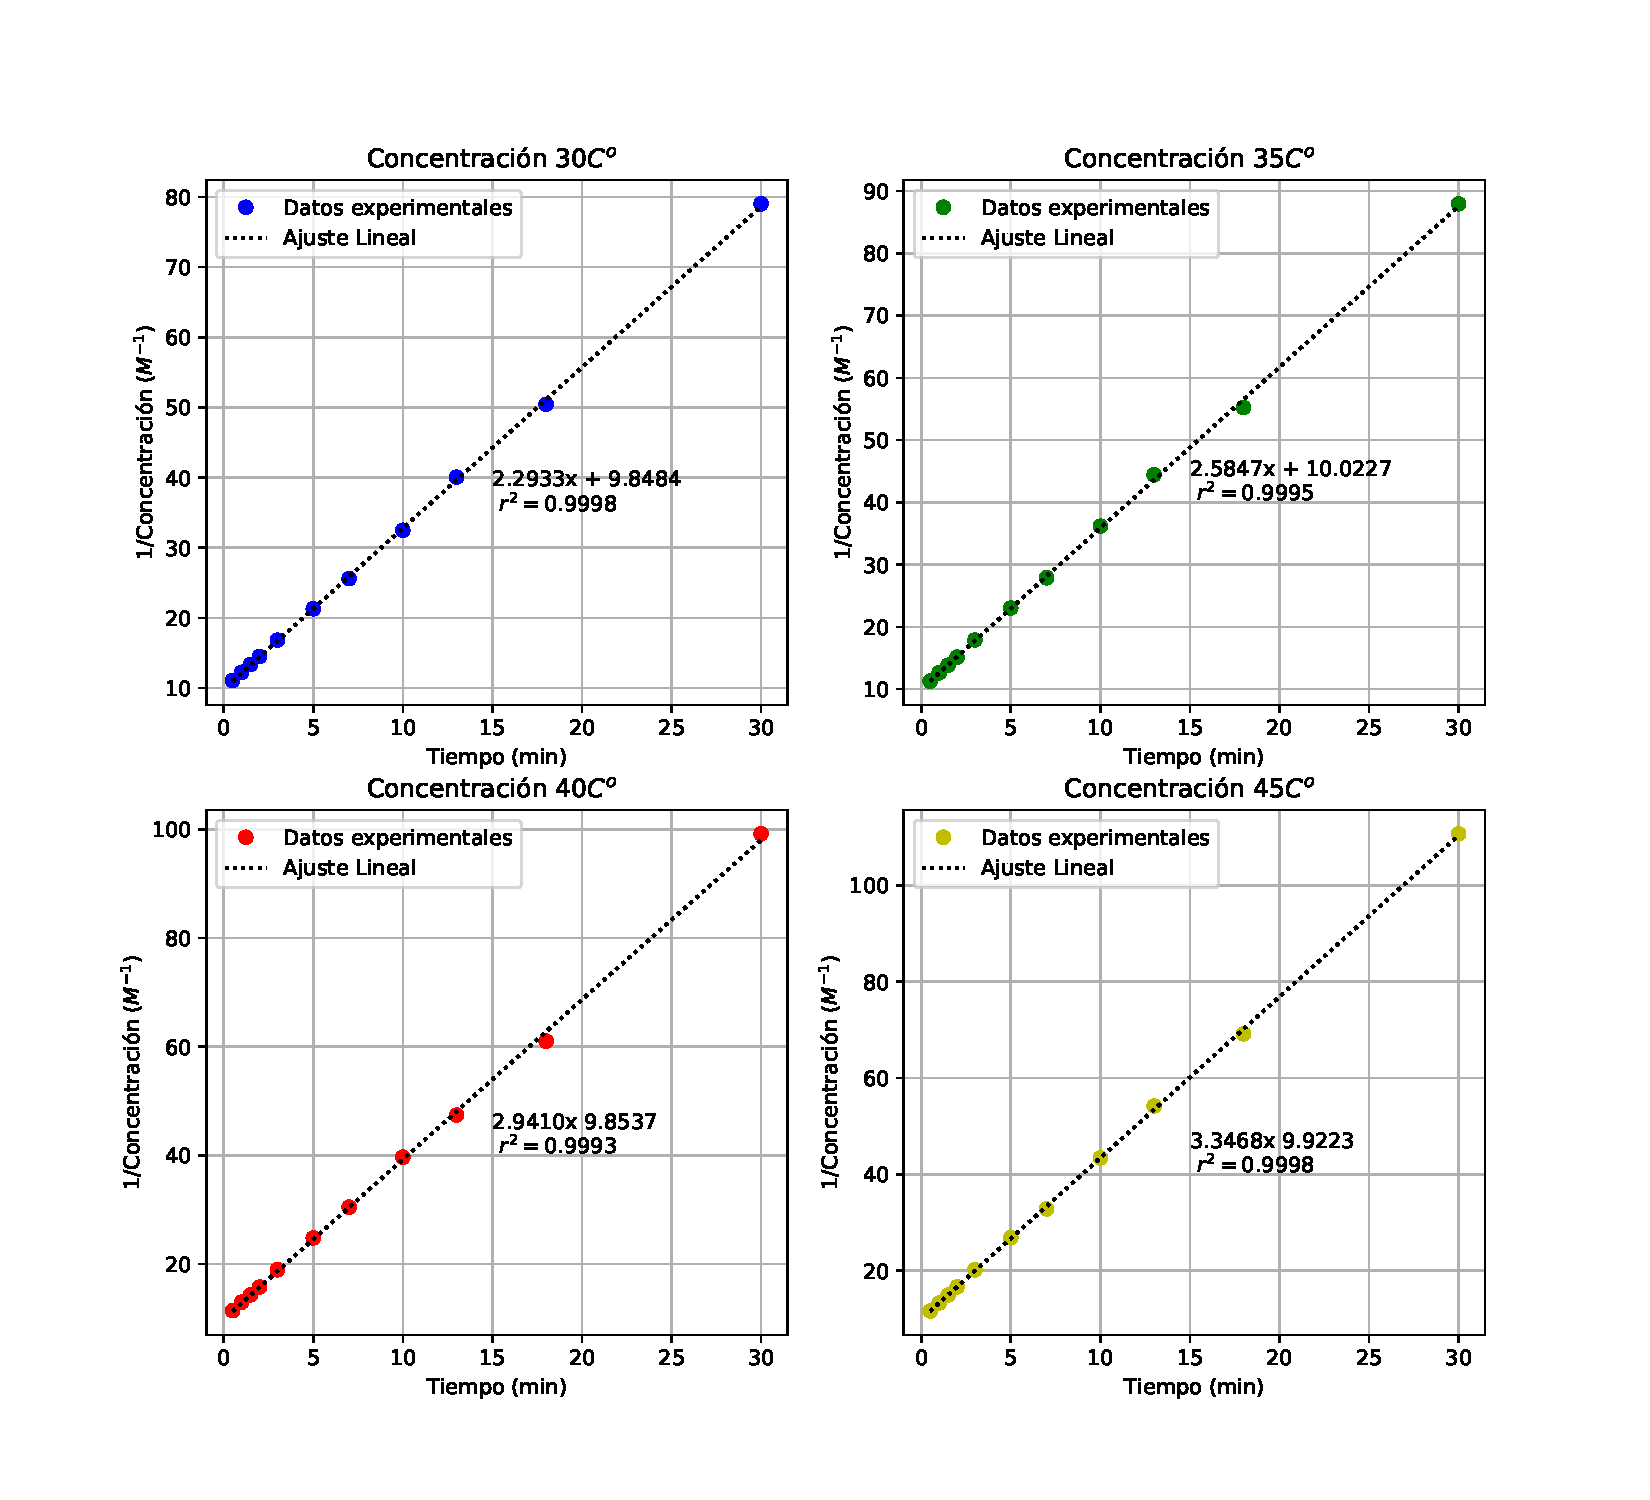
\includegraphics[scale=0.65]{Figuras/Ctodos.pdf}
    \caption{Diagrama de la pr\'{a}ctica}
\end{figure}



%begin{figure}[H]
%         \centering
%         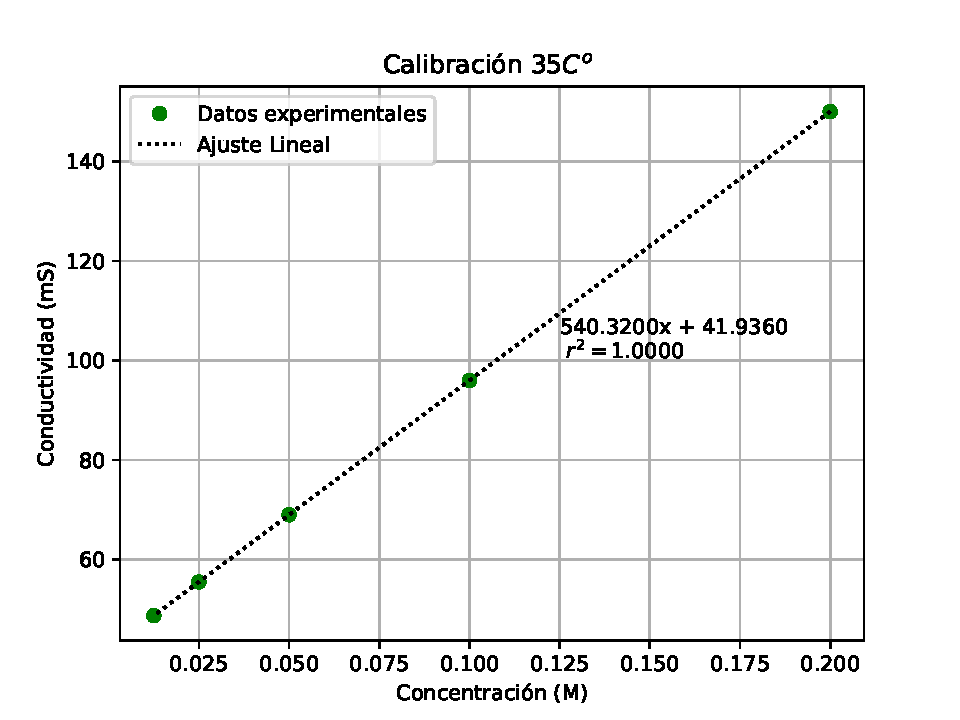
\includegraphics[scale=1]{Figuras/calibracion_35.pdf}
%#         \caption{Diagrama de la pr\'{a}ctica}
%#\end{figure}


%\begin{figure}[H]
%         \centering
%         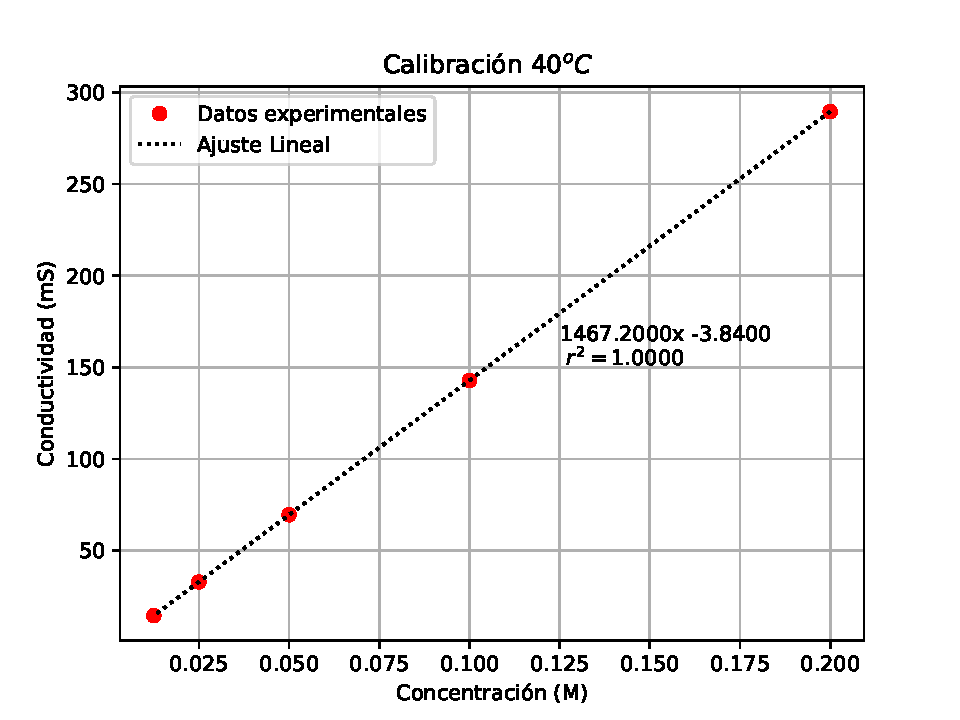
\includegraphics[scale=1]{Figuras/calibracion_40.pdf}
%         \caption{Diagrama de la pr\'{a}ctica}
%\end{figure}



%\begin{figure}[H]
%         \centering
%         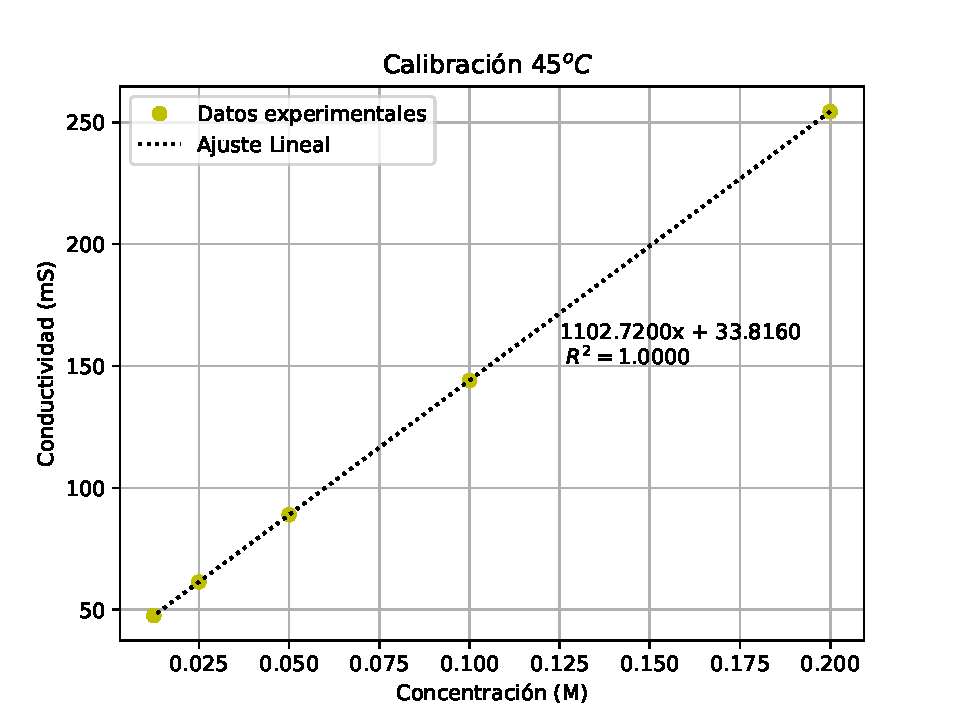
\includegraphics[scale=1]{Figuras/calibracion_45.pdf}
%         \caption{Diagrama de la pr\'{a}ctica}
%\end{figure}



%\begin{figure}[H]
%         \centering
%         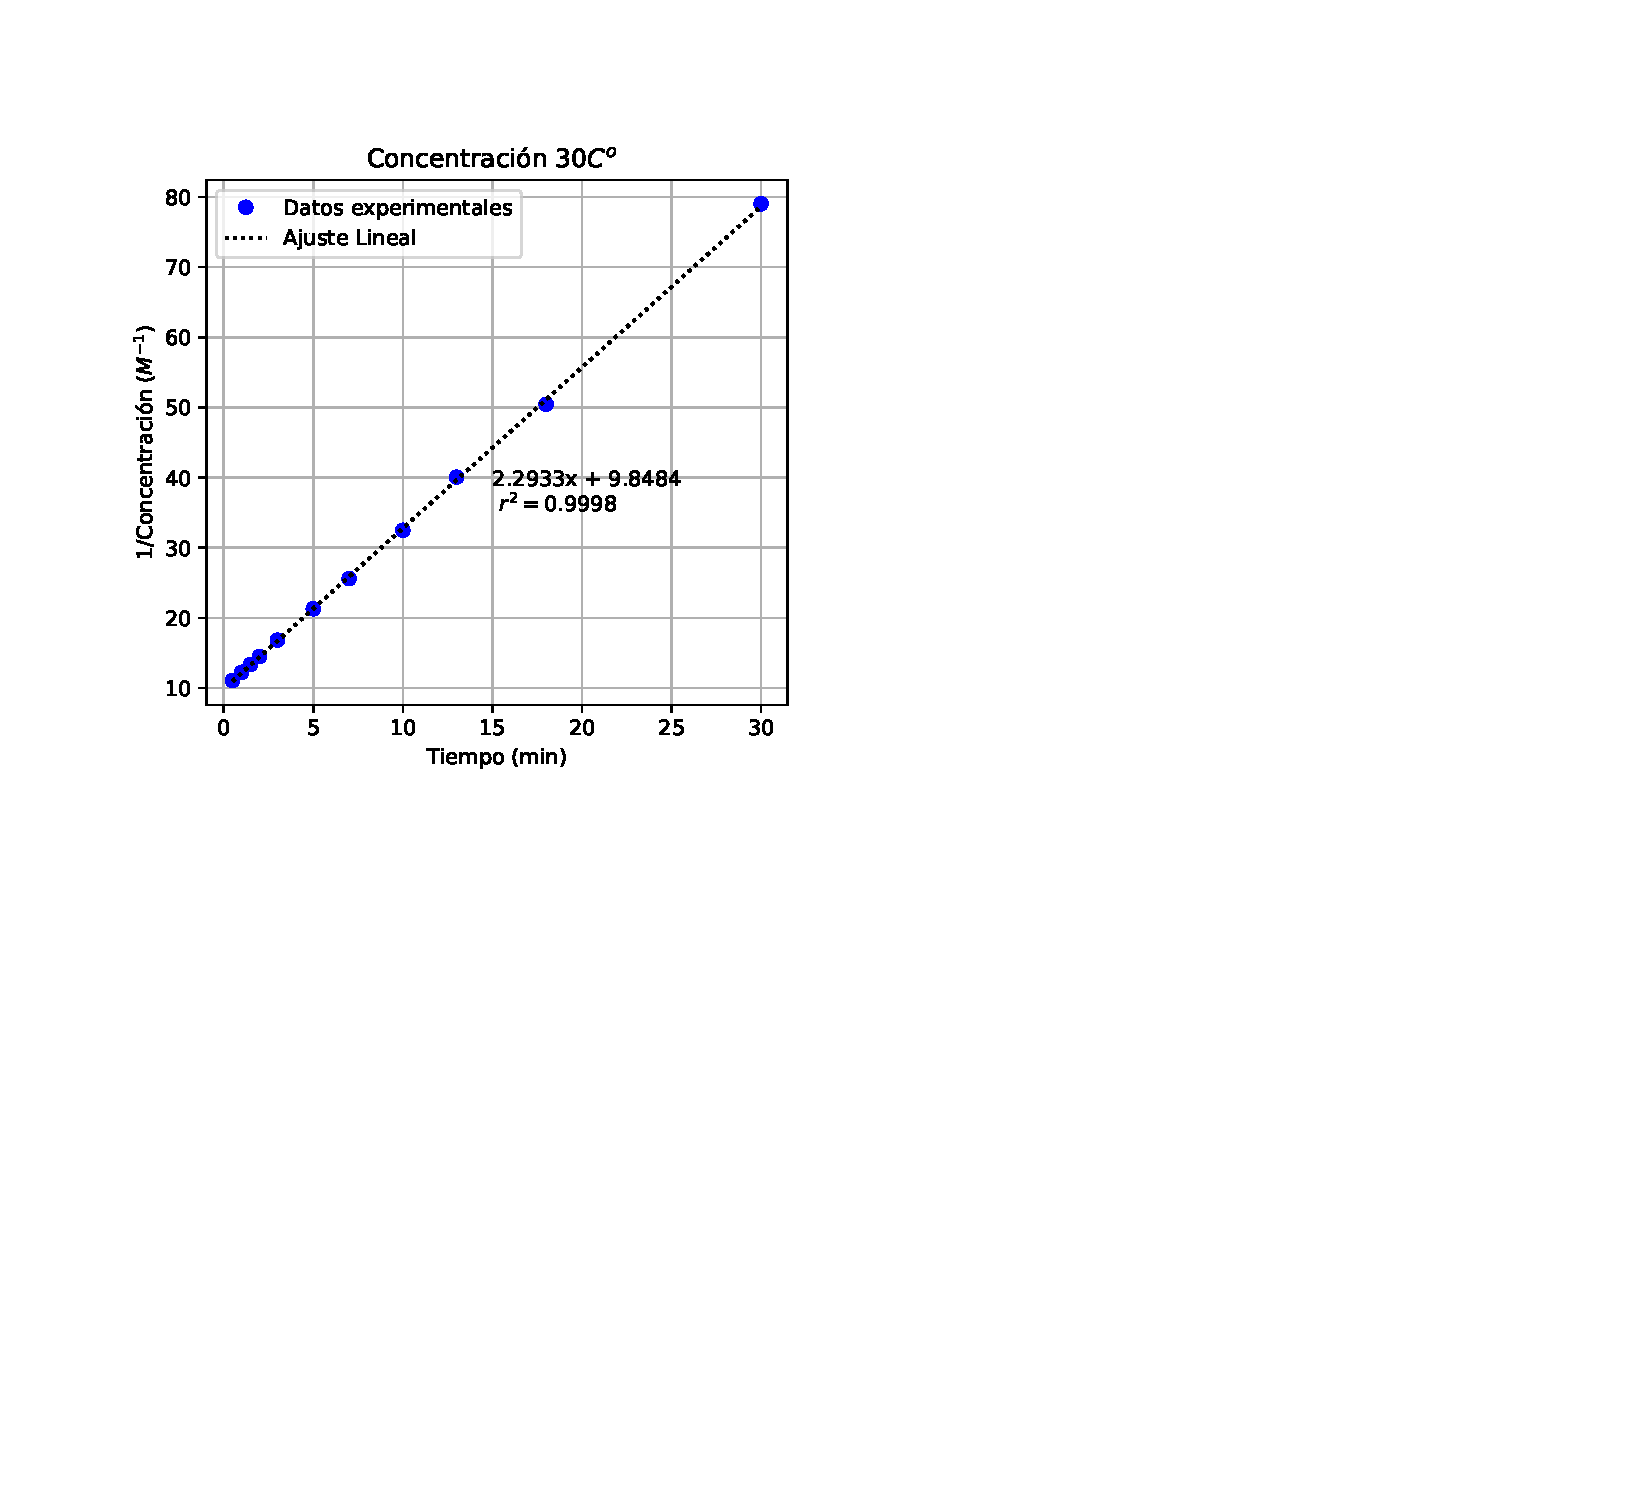
\includegraphics[scale=1]{Figuras/C_30.pdf}
%         \caption{Diagrama de la pr\'{a}ctica}
%\end{figure}


%\begin{figure}[H]
%         \centering
%         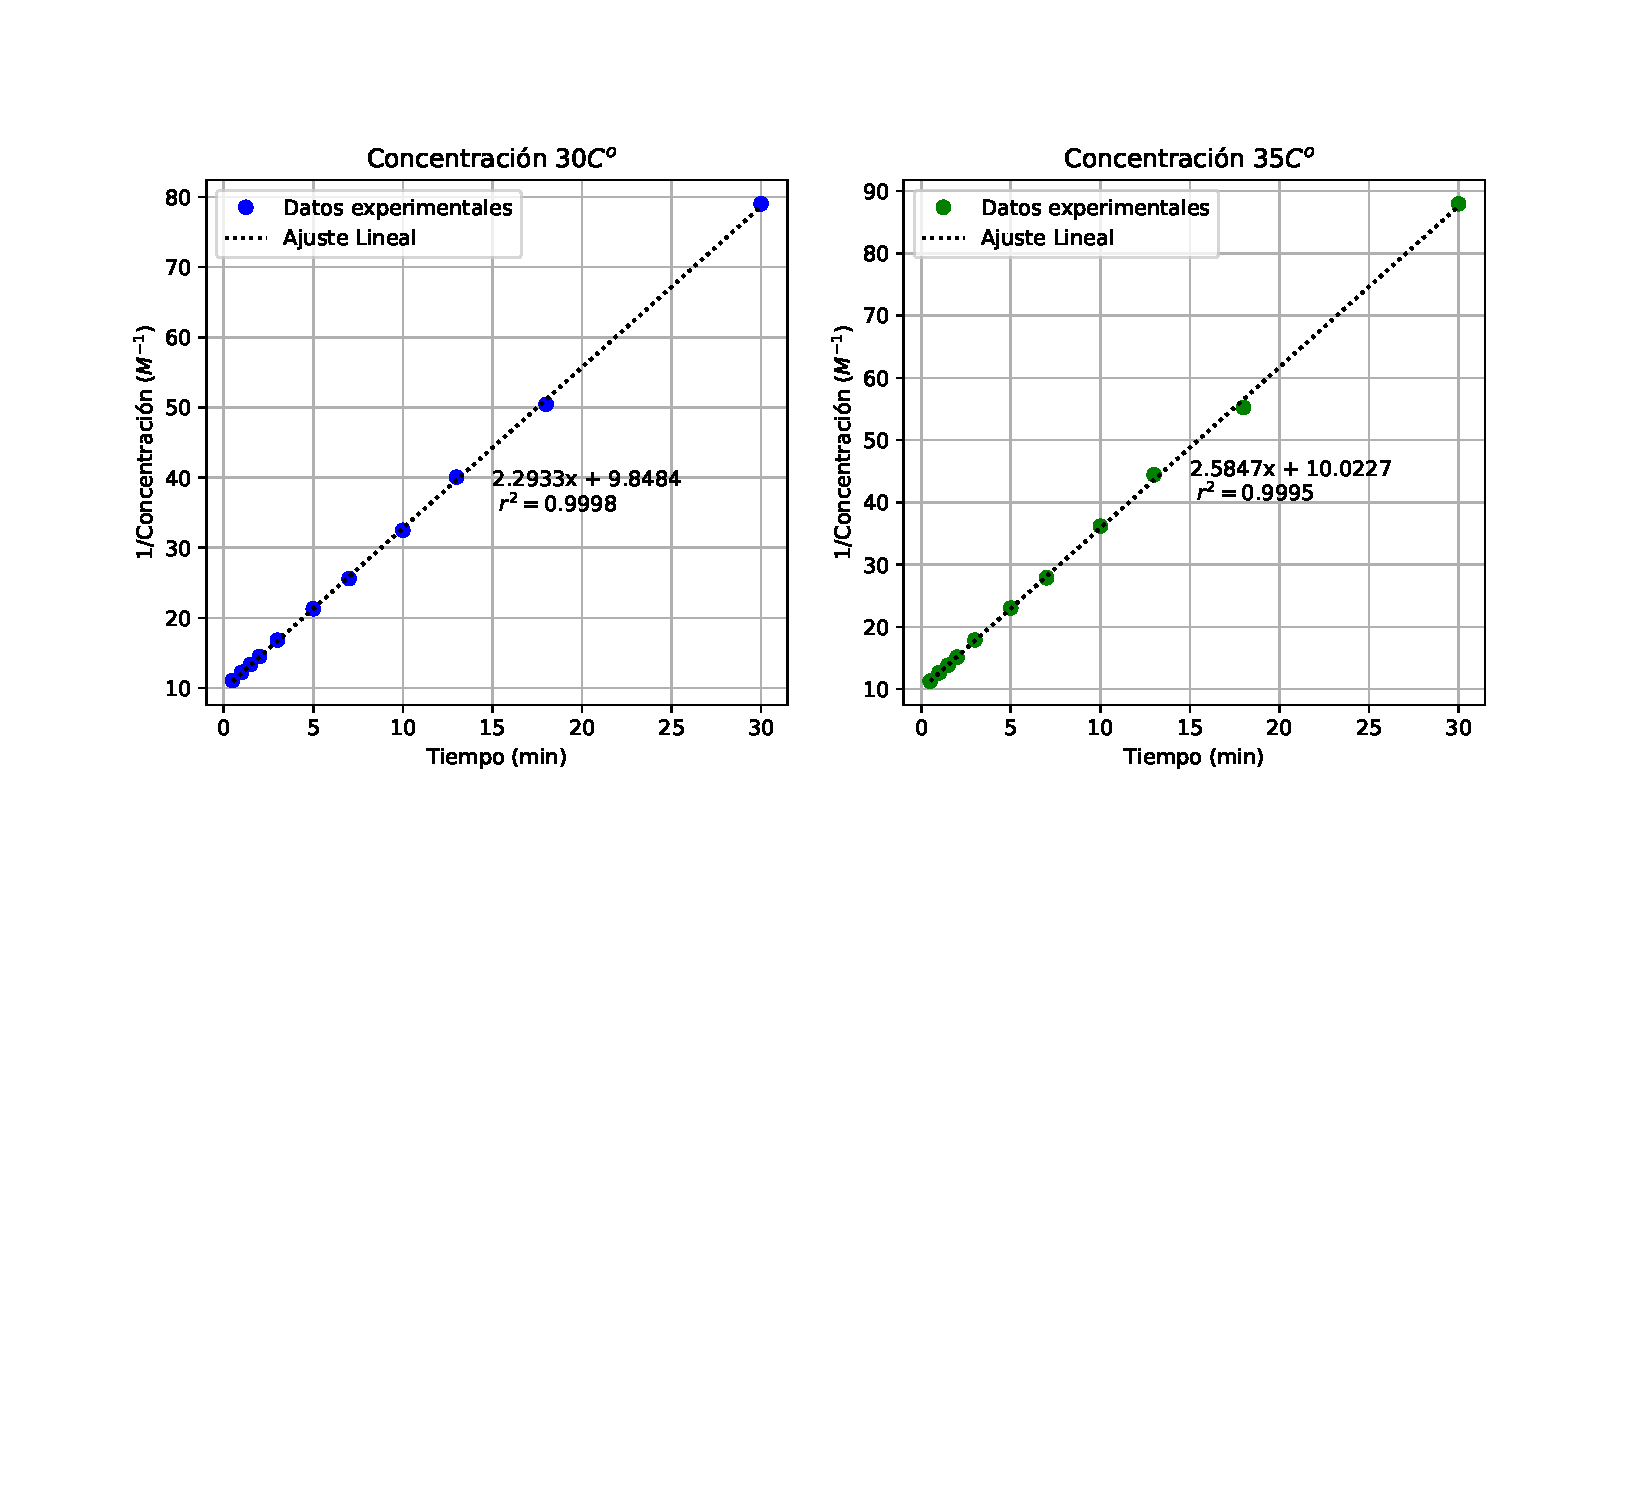
\includegraphics[scale=1]{Figuras/C_35.pdf}
%         \caption{Diagrama de la pr\'{a}ctica}
%\end{figure}


%\begin{figure}[H]
%         \centering
%         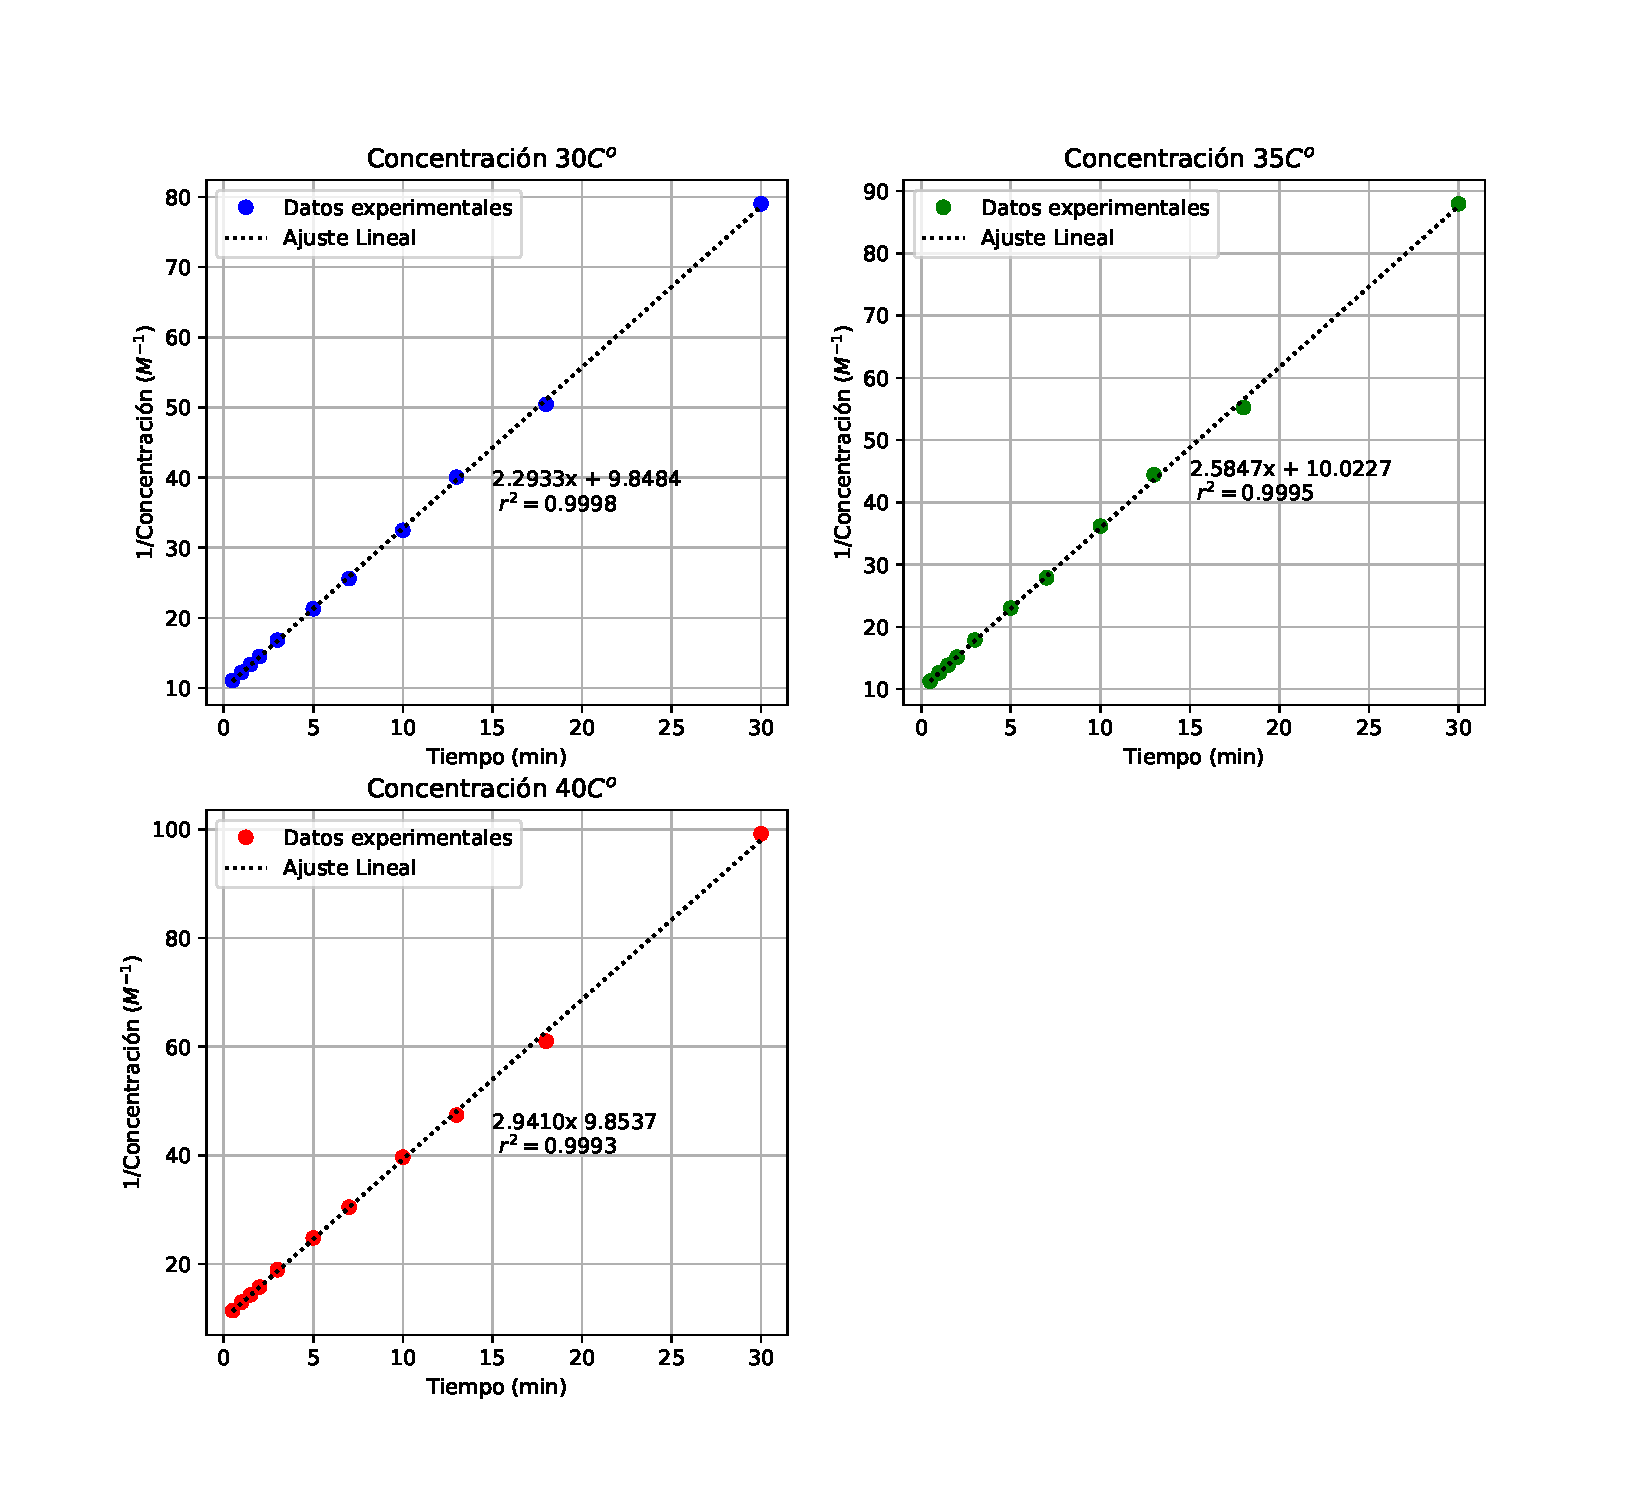
\includegraphics[scale=1]{Figuras/C_40.pdf}
%         \caption{Diagrama de la pr\'{a}ctica}
%\end{figure}


%\begin{figure}[H]
%         \centering
%         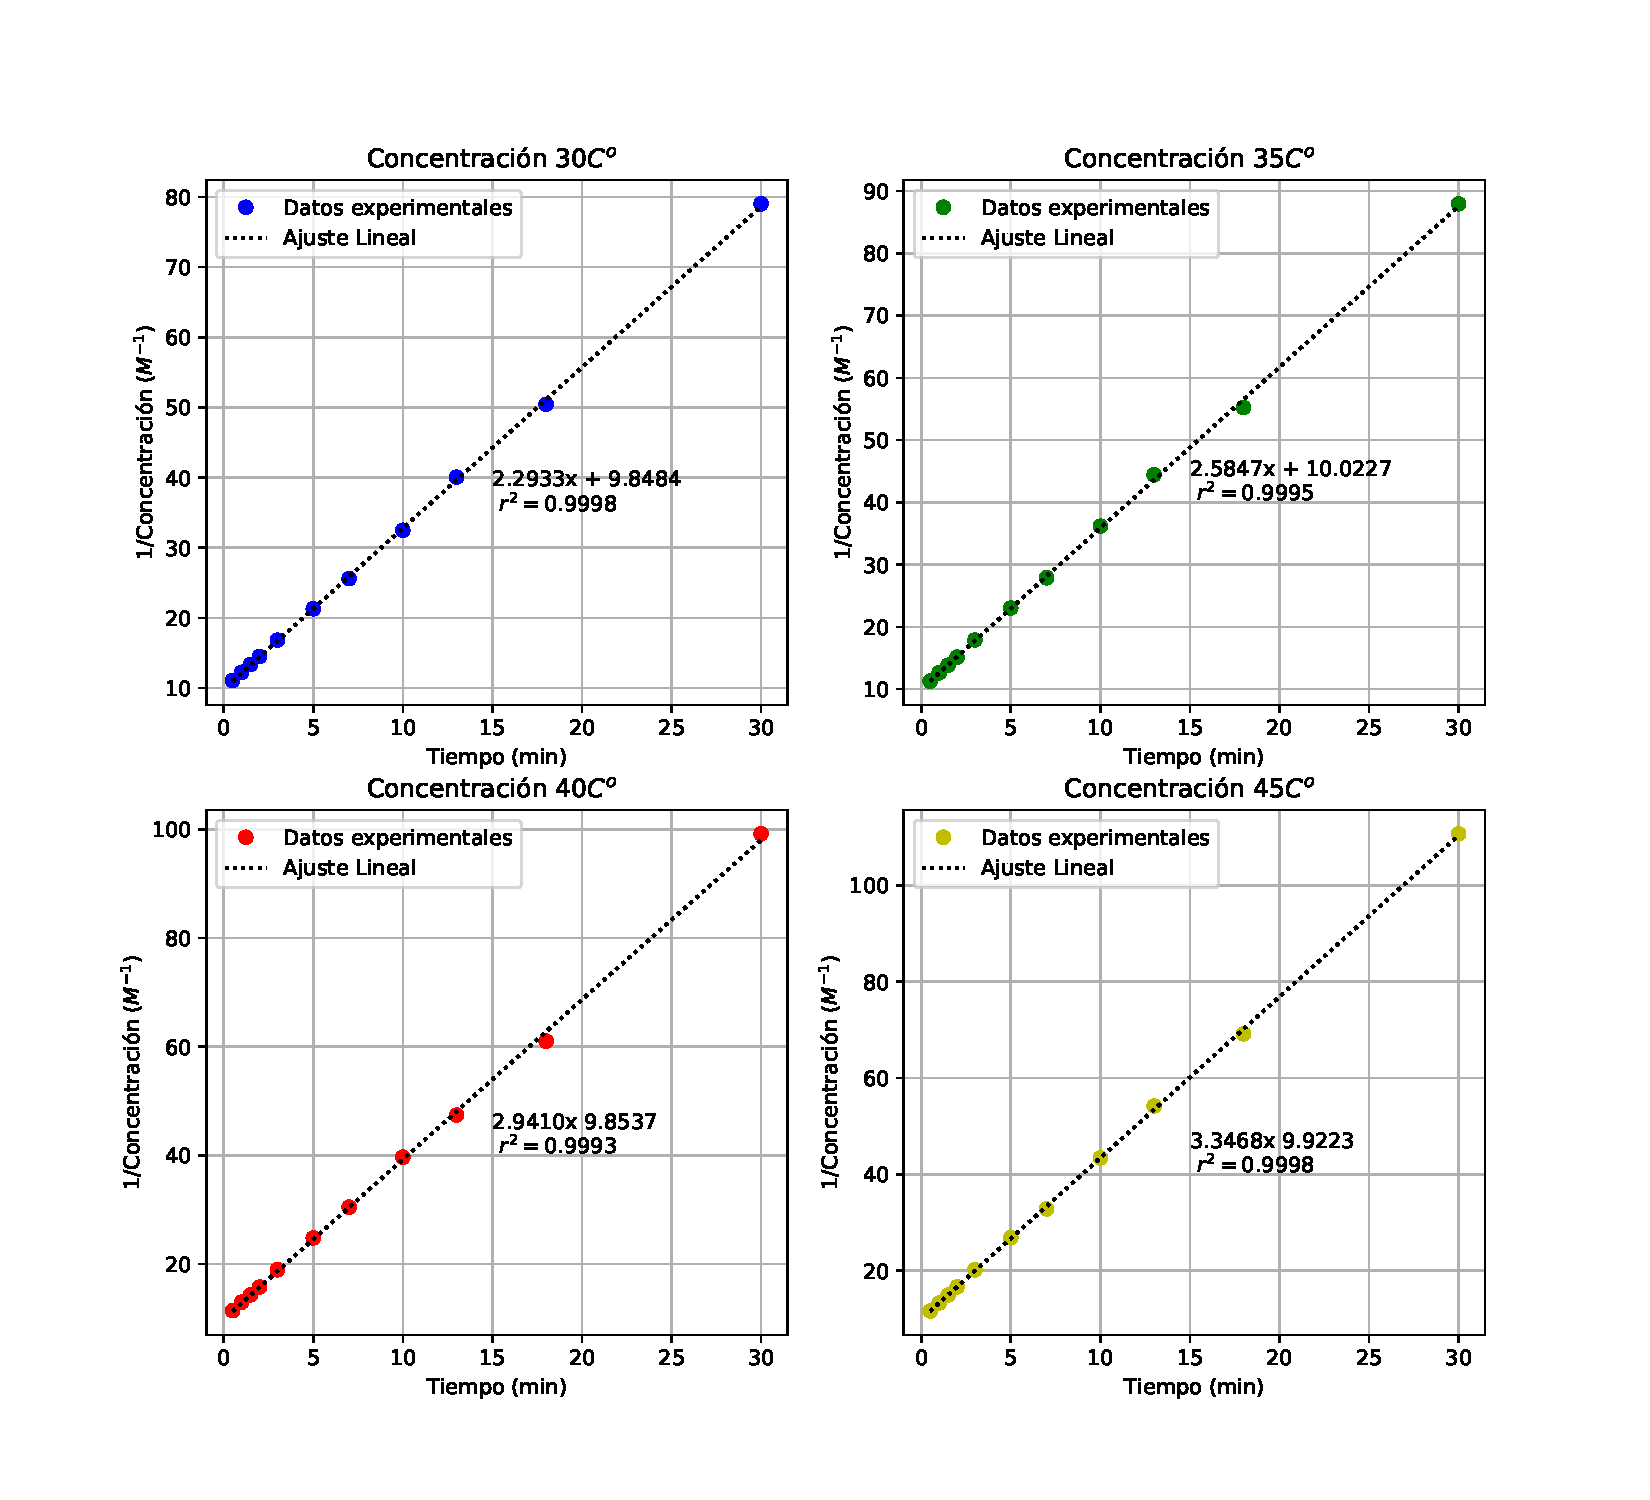
\includegraphics[scale=1]{Figuras/C_45.pdf}
%         \caption{Diagrama de la pr\'{a}ctica}
%\end{figure}

%\end{commet}




\begin{figure}[H]
         \centering
         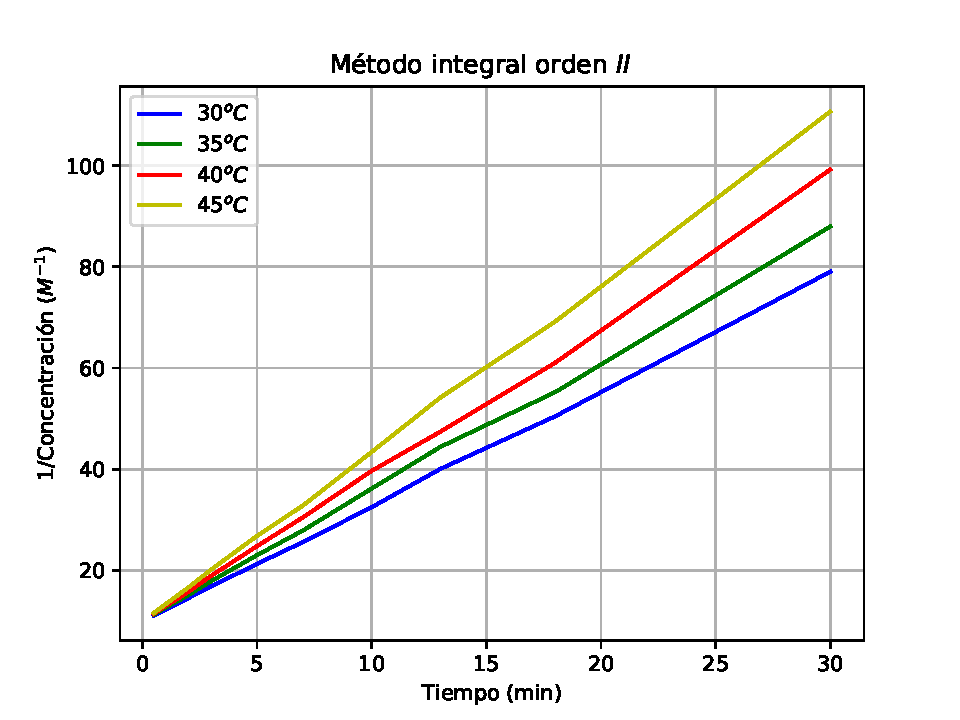
\includegraphics[scale=1]{Figuras/concentracion_todos.pdf}
         \caption{Diagrama de la pr\'{a}ctica}
\end{figure}


\begin{figure}[H]
         \centering
         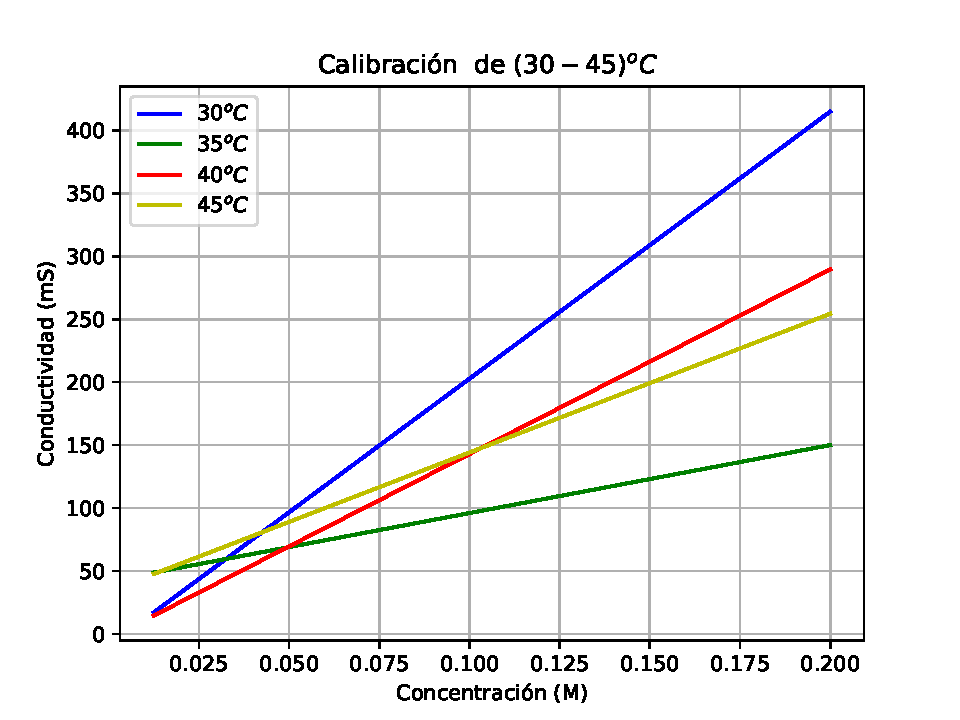
\includegraphics[scale=1]{Figuras/calibracion_todos.pdf}
         \caption{Diagrama de la pr\'{a}ctica}
\end{figure}





\end{document}
